\documentclass[tikz,border=6pt]{standalone}
\usepackage{pgfplots}
\pgfplotsset{compat=1.18}
\definecolor{demand}{HTML}{1F4E79}
\definecolor{mr}{HTML}{7EA6C8}
\definecolor{mc}{HTML}{B23A32}
\definecolor{point}{HTML}{C5161D}
\definecolor{profitA}{HTML}{97D4A4}
\definecolor{profitB}{HTML}{E98B73}
\begin{document}
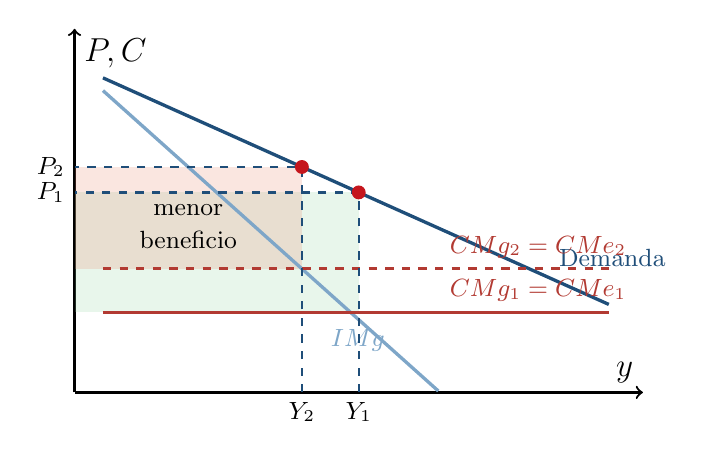
\begin{tikzpicture}
\begin{axis}[width=8.8cm,height=6.2cm,axis lines=middle,xmin=0,xmax=10,ymin=0,ymax=10,xtick=\empty,ytick=\empty,xlabel={$y$},ylabel={$P,C$},axis line style={->,thick},label style={font=\large},tick style={draw=none},clip=false]
\path[fill=profitA,opacity=.22] (axis cs:0,2.2) rectangle (axis cs:5,5.5);
\path[fill=profitB,opacity=.22] (axis cs:0,3.4) rectangle (axis cs:4,6.2);
\addplot[domain=.5:9.4,samples=2,very thick,demand] {9-.7*x} node[pos=.88,above right,font=\small] {Demanda};
\addplot[domain=.5:6.4,samples=2,very thick,mr] {9-1.4*x} node[pos=.76,below,font=\small] {$IMg$};
\addplot[domain=.5:9.4,samples=2,very thick,mc] {2.2} node[pos=.86,above,font=\small] {$CMg_1=CMe_1$};
\addplot[domain=.5:9.4,samples=2,very thick,mc,dashed] {3.4} node[pos=.86,above,font=\small] {$CMg_2=CMe_2$};
\addplot[dashed,thick,demand] coordinates {(5,0) (5,5.5) (0,5.5)};
\addplot[dashed,thick,demand] coordinates {(4,0) (4,6.2) (0,6.2)};
\addplot[only marks,mark=*,mark size=2.3pt,point] coordinates {(5,5.5) (4,6.2)};
\node[left,font=\small] at (axis cs:0,5.5) {$P_1$};
\node[left,font=\small] at (axis cs:0,6.2) {$P_2$};
\node[below,font=\small] at (axis cs:5,0) {$Y_1$};
\node[below,font=\small] at (axis cs:4,0) {$Y_2$};
\node[font=\small] at (axis cs:2,4.2) {beneficio};
\node[font=\small] at (axis cs:2,5.0) {menor};
\end{axis}
\end{tikzpicture}
\end{document}
